\documentclass{controle}
\usepackage{main}

\title{Variables aléatoires : Entraînement}
\author{TSTMG1}
\date{Chapitre 5 : Variables aléatoires}

\begin{document}
\titleandname{}
\instructions

\begin{questions}
\titledquestion{Triangle de Pascal}[5] Construire le triangle de pascal pour calculer les coefficients binomiaux $\binom{n}{k}$ pour $n \leq 10$. En déduire la valeur des coefficients suivants :
\begin{oneparchoices}
\choice $\binom{7}{2}$
\choice $\binom{8}{6}$
\choice $\binom{10}{8}$
\end{oneparchoices}

\vspace*{0.5cm}

\titledquestion{Pari sportif}[8] Pierrick décide de miser de l'argent sur une saison de $10$ matches du sport de son équipe favorite. 

\begin{parts}
\part[2] On s'intéresse à la probabilité que son équipe gagne un matche. Il y a deux stratégies : l'offensive et la défensive.
\begin{itemize}
\item Si la stratégie choisie est offensive, alors l'équipe a $60\%$ de chances de l'emporter; 
\item Si la stratégie choisie est défensive, alors l'équipe a $50\%$ de chances de l'emporter; 
\end{itemize} 
Pierrick réalise que l'équipe a autant de chances, au début de chaque match, de choisir la stratégie offensive ou défensive.

%:-+-+-+- Engendré par : http://math.et.info.free.fr/TikZ/Arbre/
\begin{center}
% Racine à Gauche, développement vers la droite
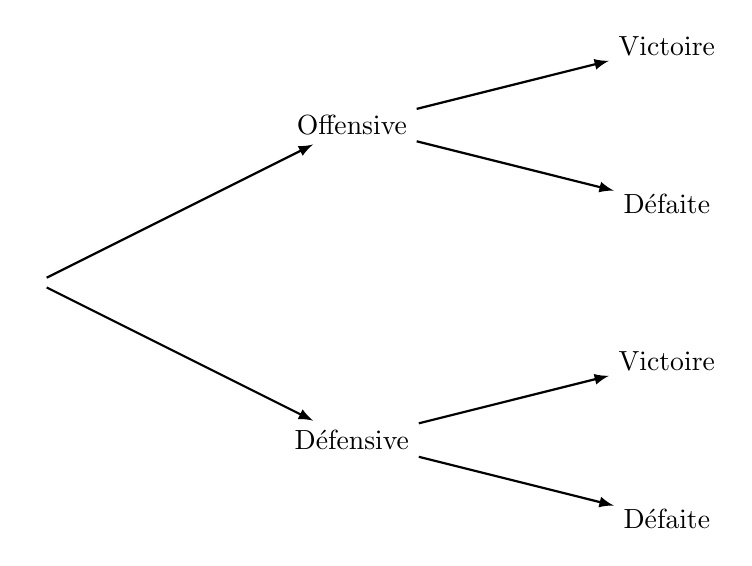
\begin{tikzpicture}[xscale=1,yscale=1]
% Styles (MODIFIABLES)
\tikzstyle{fleche}=[->,>=latex,thick]
\tikzstyle{noeud}=[]
\tikzstyle{feuille}=[]
% Dimensions (MODIFIABLES)
\def\DistanceInterNiveaux{4}
\def\DistanceInterFeuilles{2}
% Dimensions calculées (NON MODIFIABLES)
\def\NiveauA{(0)*\DistanceInterNiveaux}
\def\NiveauB{(1)*\DistanceInterNiveaux}
\def\NiveauC{(2)*\DistanceInterNiveaux}
\def\InterFeuilles{(-1)*\DistanceInterFeuilles}
% Noeuds (MODIFIABLES : Styles et Coefficients d'InterFeuilles)
\node[noeud] (R) at ({\NiveauA},{(1.5)*\InterFeuilles}) {};
\node[noeud] (Ra) at ({\NiveauB},{(0.5)*\InterFeuilles}) {Offensive};
\node[feuille] (Raa) at ({\NiveauC},{(0)*\InterFeuilles}) {Victoire};
\node[feuille] (Rab) at ({\NiveauC},{(1)*\InterFeuilles}) {Défaite};
\node[noeud] (Rb) at ({\NiveauB},{(2.5)*\InterFeuilles}) {Défensive};
\node[feuille] (Rba) at ({\NiveauC},{(2)*\InterFeuilles}) {Victoire};
\node[feuille] (Rbb) at ({\NiveauC},{(3)*\InterFeuilles}) {Défaite};
% Arcs (MODIFIABLES : Styles)
\draw[fleche] (R)--(Ra);
\draw[fleche] (Ra)--(Raa);
\draw[fleche] (Ra)--(Rab);
\draw[fleche] (R)--(Rb);
\draw[fleche] (Rb)--(Rba);
\draw[fleche] (Rb)--(Rbb);
\end{tikzpicture}
\end{center}
%:-+-+-+-+- Fin

\begin{subparts}
\subpart Compléter l'arbre de probabilité ci-dessus avec les éléments de l'énoncé.
\subpart Justifier que la probabilité que cette équipe gagne un match est $p = 0,55$.
\end{subparts}
\part[6] Pour la suite, on suppose que chaque match dans une saison est indépendant, et que tous ont la même probabilité $p$ de gagner. On note $X$ le nombre de matches gagnés lors d'une saison.
\begin{subparts}
\subpart[1] Justifier que $X$ suit une loi binomiale de paramètres $n$ et $p$ que l'on explicitera.
\subpart[1] En déduire la formule permettant de calculer $P(X = 8)$ (On utilisera les valeurs obtenues à l'exercice 1).
\subpart[1] Même question pour $P(X = 3)$.
\subpart[2] Donner la formule permettant de calculer $P(X \geq 8)$. 
\subpart[1] Donner la formule permettant de calculer l'espérance $E(X)$. Quel est le nombre moyen de matches gagnés lors d'une saison ?
\end{subparts}
\end{parts}


\titledquestion{Jeu de l'identique}[7]

On s'intéresse au jeu suivant : le joueur mise \num{5}€, puis lance deux dés (un rouge et un bleu) équilibrés à six faces numérotées de $1$ à $6$. Il gagne \num{11}€ s'il fait un double (un double $4$ par exemple), et \num{7}€ si les valeurs des résultats des deux dés sont distants de $1$ (Par exemple, si le dé rouge renvoie $3$ et le dé bleu renvoie $4$). Dans tous les autres cas, le joueur ne gagne rien.

On note $X$ le gain après une partie du jeu (en comptant la mise de départ).

\begin{parts}
\part[2] Compléter le tableau suivant avec les gains pour chaque configuration.
\begin{center}
\begin{tblr}{hlines,vlines, rows={0.6cm,m,mode=math}, columns={0.6cm,c}, column{1}={2.5cm,c,mode=text}, row{1}={2cm,mode=text}}
\diagbox[width=2.5cm, height=2cm]{Rouge}{Bleu}&1&2&3&4&5&6\\
1&&&&&&-5\\
2\\
3\\
4\\
5\\
6\\
\end{tblr}
\end{center}
\part[1] Donner la probabilité que le gain soit $-5$, c'est-à-dire $P(X = -5)$.
\part[1] Procéder de la même manière sur les autres gains possibles afin de déterminer la loi de $X$ en complétant le tableau suivant.
\begin{center}
\begin{tblr}{hlines, vlines, rows={m,mode=math}, columns={c,0.6cm}, column{1} = {2cm}}
k&-5&&\\
P(X=k)&&&
\end{tblr}
\end{center}
\part[1] En déduire l'espérance de $X$, $E(X)$.
\part[2] On suppose que lorsque que les deux dés renvoient des résultats distants de $1$, le jeu rapporte $x$€, avec $x$ un nombre réel. Quelle doit être la valeur de $x$ pour que le jeu soit équitable, c'est-à-dire pour que $E(X)=0$ ?

\end{parts}
\end{questions}
\end{document}